\documentclass[]{article}

\usepackage{amsmath,amsfonts,amssymb}
\usepackage{listings}
\usepackage{graphicx}
\usepackage{authblk}
\usepackage[top=2cm, bottom=2cm, left=2cm, right=2cm]{geometry}

% add by Chunlong Luo
\usepackage{amssymb}
\usepackage{bm}
%\DeclareMathOperator*{\min}{min}
\DeclareMathOperator*{\argmin}{argmin}
% add by Chunlong Luo

%\makeatletter
%\let\@fnsymbol\@arabic
%\makeatother




\title{Variable Selection For Discrete Competing Risks Models}
\date{\today}
\author{%
   Jingwei Zhang\thanks{skykiny@outlook.com},
   Lupengkong, 
   Chunlong Luo,
   Quanfeng Yang,
   Yiqing Lu
}
\begin{document}
    \maketitle
    
    \section{Introduction}
    \subsection{Applied problem}
        \paragraph{}In survival or, more general, time-to-event regression analysis, one aims at quantifying the effects of explanatory variables on the duration time. Simple survival analysis considers one terminating event, for example death in disease studies. In many applications, however, duration can end by the occurrence of several possible events. For example, in unemployment studies the time of unemployment ends if an individual takes a full-time job, a part-time job, or retires.
    \subsection{Statistical problem}
        \paragraph{}Modeling of the event times in the presence of multiple outcomes is usually referred to as competing risks modeling. Alternatively, one also speaks of competing events, competing causes or failures to convey that several events compete with each other to be observed.
    \subsection{Existing methods}
        \paragraph{}Most of the literature for competing risks considers the case of continuous time. If time is discretely observed, ties may cause problems in the estimation procedure and the model might become inappropriate, especially for a low number of time periods.
        \paragraph{}Competing risks models for discrete time have been considered, but without referring to the problem of variable selection. While in simple survival models the impact of an explanatory variable is typically contained in one parameter, in competing risk models there is always a group of parameters that are linked to one predictor. This special feature calls for specific variable selection techniques.
        \paragraph{}Conventional variable selection methods are forward- and backward-stepwise selection. However, these methods are frequently unstable and cannot be recommended. More current alternative model selection approaches use regularization techniques. In particular, penalization is nowadays widely used to regularize estimates by adding a penalty term to the log-likelihood. One of the oldest penalization methods is the ridge method. An alternative penalty approach that has become very popular is the lasso Tibshirani (1996) .Several improvements for the lasso method have been proposed in the last decade, for example the group lasso, the adaptive lasso, SCAD, the elastic net and the Dantzig selector.
        \paragraph{}However, these methods are designed for models with univariate response. If used in multiple response models as the competing risks model they are not efficient in terms of variable selection because the effect of one predictor variable is represented by several parameters. Hence, there is a difference in providing variable selection and parameter selection. Variable selection is obtained only if all the parameters belonging to a variable are simultaneously set to zero. The available penalty techniques for multinomial logit model. More recently, alternatives that enforce variable selection instead of variable select in multiple response models were proposed.
    \subsection{New contribution}
        \paragraph{}When modeling cause-specific hazard rates in competing risk model, each explanatory variable is linked to a group of parameters. A new penalization method is proposed in this article that enforces the simultaneous shrinkage of parameters belonging to such a group. A parameter group even can be completely removed from the model yielding variable selection instead of
        parameter selection. Moreover, the proposed method allows that parameters representing the cause-specific baseline hazards vary over time. In order to avoid that adjacent parameters of the baseline effects have completely different values, an additional penalty
        term is incorporated that steers the smoothness of the baseline effects.
        \paragraph{}We apply this method to one problems, the congressional careers of members of the US congress.
    
    
    
    
    \section{Competing Risk Model for Discrete Time} % Model
    \subsection{The Discrete Competing Risk Model}
    \paragraph{} Let $\mathbf{x}$ be the covariates of one object. Competing risk model determines to analysis the influence of $\mathbf{x}$ on the happening of the several events(or causes of risks).
    \paragraph{}Let time take values from $\{1,\dots,k\}$ and let $q = k-1$. Discrete time $T \in \{1,\dots,k\}$ means that
    $T = t$ is observed if failure occurs on time $t$. If time values result from intervals, one has $k$ underlying intervals $[a_0, a_1),[a_1, a_2),\dots,[a_{q−1}, a_q), [a_q, \infty)$, where typically $a_0 = 0$ is assumed and $a_q$ denotes the final follow-up. $T = t$ is observed if failure occurs within the time interval $[a_{t−1}, a_t)$.
    
    \paragraph{}Let the distinct terminating causes be denoted by $R \in \{1,\dots, m\}$. Then the cause-specific discrete hazard function resulting from cause $r$ is determined by the conditional probability
    \begin{equation}
        \lambda_r(t|\mathbf{x}) = P(T = t, R = r | T \geq t, \mathbf{x})
    \end{equation}
    where $r = 1,\dots,m$ and $t = 1,\dots,q$. The $m$ hazard functions sum up to an overall hazard function
    \begin{equation}
        \lambda(t|\mathbf{x}) = \sum_{r = 1}^{m} \lambda_r(t|\mathbf{x}) = P(T = t | T \geq t, \mathbf{x})
    \end{equation}
    The survival function, which indicates the unconditional probability of no event happening on time collection $\{1,\dots,t\}$, is given by
    \begin{equation}
        S(t|\mathbf{x}) = P(T > t | \mathbf{x}) = \prod_{j = 1}^{t} (1-\lambda(j|\mathbf{x}))
    \end{equation}
    The unconditional probability of one event happening on time $t$ is given by
    \begin{equation}
        P(T= t|\mathbf{x}) = \lambda(t|\mathbf{x}) \prod_{j = 1}^{t-1} (1-\lambda(j|\mathbf{x})) = \lambda(t|\mathbf{x}) S(t-1|\mathbf{x})
    \end{equation}
    If a object reaches time $t-1$, there are $m + 1$ possible outcomes, transition to one of the $m$ target events or survival. The corresponding conditional
    probabilities are given by 
    \begin{equation}
        \lambda_1(t|\mathbf{x}),\dots,\lambda_m(t|\mathbf{x}), 1-\lambda(t|\mathbf{x})
    \end{equation}
    where $1-\lambda(t|\mathbf{x})$ is the probability for survival(no event happens).
    \paragraph{}Therefore, given an individual reaches time $t-1$, the hazards can be modeled by the multinomial logit model given by
    \begin{equation}\label{logit_model_r}
        \lambda_r(t|\mathbf{x}) = \frac{ \exp{ (\beta_{0tr}+\mathbf{x}^\mathsf{T} \mathbf{\gamma_r} ) } }{ 1+ \sum_{s=1}^{m} \exp{ (\beta_{0ts}+\mathbf{x}^\mathsf{T} \mathbf{\gamma_s}) }  }
    \end{equation}
    where $t = 1,\dots, q$, and $r = 1,\dots, m$. We define $\eta_itr = \beta_{0tr}+\mathbf{x}^\mathsf{T} \mathbf{\gamma_r}$. Then the parameters $\beta_{01r}, \dots, \beta_{0qr}$ determine the
    cause-specific baseline hazard functions and $\mathbf{\gamma_r}$ contains the cause-specific effects of
    covariates. Conditional probability of survival is implicitly determined by
    \begin{equation}\label{logit_model_0}
        \lambda_0(t|\mathbf{x})=P(T>t|T\geq t,\mathbf{x}) = 1 - \sum_{r=1}^{m} \lambda_r(t|\mathbf{x}) = \frac{ 1 }{ 1+ \sum_{s=1}^{m} \exp{ (\beta_{0ts}+\mathbf{x}^\mathsf{T} \mathbf{\gamma_s}) }  }
    \end{equation}
    Let $R = 0$ denote the conditional survival, the conditional
    probabilities are given by $\lambda_0(t|\mathbf{x}) = P(T > t|T \geq t, \mathbf{x}), \lambda_1(t|\mathbf{x}),\dots, \lambda_m(t|\mathbf{x})$, which sum
    up to one.
    
    \subsection{Estimation}
    \paragraph{}Let data be given by $(t_i,r_i,\delta_i, \mathbf{x}_i)$, $i = 1,\dots,n$, where $t_i = min(Ti,Ci)$ is the observed discrete time, which is the minimum of survival time $T_i$ and censoring time $C_i$. We always
    assume random censoring, that is, $T_i$ and $C_i$ are assumed to be independent. Moreover,$r_i \in \{1,\dots,m\}$ indicates the type of the terminating event, $\mathbf{x}_i$ is the covariate vector and $\delta_i$ denotes the censoring indicator with
    \begin{align}
        \delta_i = \begin{cases}
        1, &\quad \text{if event occured on time }t_i \\
        0, &\quad \text{if it censores on time }t_i
        \end{cases}
    \end{align}
    Under the assumption that censoring does not depend on the parameters that determine
    the survival time (non-informative censoring), the likelihood contribution of the i-th observation is
    \begin{align}
    \begin{split}
        L_i &= P(T_i = t_i,R_i = r_i|\mathbf{x})^{\delta_i}P(T_i > t_i|\mathbf{x})^{1-\delta_i}  \\
        &=\lambda_{r_i}(t_i|\mathbf{x}_i)^{\delta_i}
          (1-\lambda(t_i|\mathbf{x}_i))^{1-\delta_i}
          \prod_{t=1}^{t_i-1}(1-\lambda(t|\mathbf{x}_i)) \label{log liklihood using delta}
    \end{split}
    \end{align}
    Let $R_t = \{i : t \leq t_i\}$ be the risk set containing all objects who are at risk on time $t$. For an alternative form of the likelihood, indicators for the transition to the
    next period are defined by
    \begin{align}
        y_{itr} = \begin{cases}
            1, &\quad \text{if event of type }r\text{ occured on time }t \\
            0, &\quad \text{if event of type }r\text{ did not occure on time }t
        \end{cases}
    \end{align}
    and
    \begin{align}
    y_{it0} = \begin{cases}
    1, &\quad \text{if no events occured on time }t \text{ (survive)} \\
    0, &\quad \text{if one of the } m\text{ events occures on time }t
    \end{cases}
    \end{align}
    where $i \in R_t$ and $r=1,\dots,m$. These indicator variables are gathered in the vector $\mathbf{y}_{it}^\mathsf{T}  = (y_{it0},y_{it1},...,y_{itm})$ denoting the response vector of object $i$, $i = 1,\dots,n$, $t = 1,\dots,t_i$. Then, the likelihood function $Li$ can be rewritten as
    \begin{align}
     L_i = \prod_{t = 1}^{t_i}  (\prod_{r = 0}^{m} \lambda_{r}(t_i|\mathbf{x}_i)^{y_{itr}}) 
    \end{align}
    The total log-liklihood is given by
    \begin{align}
        l = \sum_{i=1}^{n} \sum_{t = 1}^{t_i} \sum_{r=0}^{m}
           y_{itr} \log\lambda_r(t|\mathbf{x})
    \end{align}
    where $\lambda_r(t|\mathbf{x})$ is given by the model \eqref{logit_model_r}	and \eqref{logit_model_0}. This ML estimates can be easily computed by using statistical software for multinomial regression models.
    \section{Choice of Penalty Term} % Method
    \subsection{The original penalty term}
    \paragraph{}
    The model of the cause-specific hazard function ${\lambda _{\rm{r}}}(t|{x_i})$ has the form of parameters:
    \begin{equation}
    {\eta _{itr}} = {\beta _{0tr}} + \mathbf{x_i}^T{\gamma _r},t = 1,...q;r = 1,...,m,
    \end{equation}
    where $\mathbf{x_i}^T=(x_{i1},...,x_{ip})$ and $\gamma _r^T=(\gamma _{r1},...,\gamma _{rp})$. \\
    
    To obtain a sparse representation and in particular variable selection, the authors consider the penalized ML estimation:
    \begin{equation}
    {l_{{\zeta _1},{\zeta _2}}}({\beta _0},\gamma ) = l({\beta _0},\gamma ) - {J_{{\zeta _1},{\zeta _2}}}({\beta _0},\gamma ),
    \end{equation}
    where  $\beta_0^T=(\beta_{01}^T,...,\beta_{0m}^T)$ and $\gamma^T=(\gamma _1^T,...,\gamma _m^T)$. $l({\beta _0},\gamma )$ denotes the ordinary log-likelihood, and ${J_{{\zeta _1},{\zeta _2}}}({\beta _0},\gamma )$ stands for a penalty term that depends on scalar tuning parameters $\zeta _1$ and $\zeta _2$.\\
    
    Authors adopt lasso for variable selection. The penalty term  is given by
    \begin{equation}
    \begin{split}
    {J_{{\zeta _1},{\zeta _2}}}({\beta _0},\gamma ) &= {\zeta _1}\sum\limits_{r = 1}^m {\sum\limits_{t = 2}^q {{{({\beta _{0tr}} - {\beta _{0,t - 1,r}})}^2}} }  + {\zeta _2}\sum\limits_{j = 1}^{\rm{p}} {{\phi _{\rm{j}}}||{\gamma _{.j}}||} \\
    & = {\zeta _1}{J_1}({\beta _0}) + {\zeta _2}{J_2}(\gamma )
    \end{split}
    \end{equation}
    where $||u|| = ||u|{|_2} = \sqrt {{u^T}u}$, $ {\phi _j} = \sqrt m $ and $\gamma _{.j}^T=(\gamma _{1j},...,\gamma _{mj})$. The penalty item ${\zeta _1}{J_1}({\beta _0})$ on the baseline parameters $\beta_0$ is used to ensure that the estimated hazard rates are sufficiently smooth over time. The penalty ${\zeta _2}{J_2}(\gamma )$ is used for variable selection. A variable is removed from the model if and only if all of its effect parameters are set to zero simultaneously. Therefore, ${J_2}(\gamma ) $ makes it if $\mathbf{x_i}$ is removed only when $||{\gamma _{.j}}|| = \sqrt {{\gamma _{1j}}^2 + {\gamma _{2j}}^2 + ... + {\gamma _{mj}}^2}  = 0$ and then $\gamma _{ij}=0 $ where $i=1,2,...,m$.
    
    \subsection{Improvement for penalty item for ${J_1}(\beta_0 )$}
    \paragraph{}
    To simplify the baseline effects and reduce the number of time periods q in ${J_1}(\beta_0 )$, it is expanded in in an equidistant and  low-rank B-spline basis function, resulting in
    \begin{equation}
    {\beta _{0tr}} = \sum\limits_{s = 1}^{{d_r}} {{\alpha _{0sr}}{B_s}(t)}
    \end{equation}
    with $d_r < q$. The total penalty function can be rewritten as
    \begin{equation}
    {J_{{\zeta _1},{\zeta _2}}}({\alpha _0},\gamma ) = {\zeta _1}\sum\limits_{r = 1}^m {\sum\limits_{s = 2}^{{d_r}} {{{({\alpha _{0{\rm{s}}r}} - {\alpha _{0,s - 1,r}})}^2}} }  + {\zeta _2}\sum\limits_{j = 1}^{\rm{p}} {{\phi _{\rm{j}}}||{\gamma _{.j}}||}
    \end{equation}
    
    \subsection{The final penalty term}
    \paragraph{}
    The choice of tuning parameter $\zeta_2 $ involves a tradeoff between fewer variable selection and unbiasedness. In the light of this conflict, adaptive weights for the penalties is an optimal choice.
    \begin{equation}
    {\phi _j}^a = \frac{{\sqrt m }}{{||\gamma _{.j}^{Init}||}}
    \end{equation}
    $\gamma _{.j}^{Init}$ is the penalized estimator that results from application of penalty function above with $\zeta_2 = 0$.
    Then the penalty function be finally written as
    \begin{equation}
    {J_{{\zeta _1},{\zeta _2}}}({\alpha _0},\gamma ) = {\zeta _1}\sum\limits_{r = 1}^m {\sum\limits_{s = 2}^{{d_r}} {{{({\alpha _{0{\rm{s}}r}} - {\alpha _{0,s - 1,r}})}^2}} }  + {\zeta _2}\sum\limits_{j = 1}^{\rm{p}} {{\phi _{\rm{j}}}^a||{\gamma _{.j}}||}
    \end{equation}\\
    
    Assuming that all predictors are centered around zero and standardized to a common variance, the norm of unpenalized estimates for the parameter groups is rather large if they belong to strong predictors and small otherwise. Consequently, the corresponding penalization is small for strong predictors and large for weak predictors. However, these penalized estimators with adaptive weights can  provide consistent variable selection.
    \section{Computional Issues}% also Method
    
    \paragraph{}To estimate the parameters $\bm{\beta_0}$ and $\bm{\gamma}$,the penalized log-likelihood $l_{\zeta_1,\zeta_2}(\bm{\beta_0},\bm{\gamma})$ can be formulated as
    \begin{equation}
    (\bm{\hat{\beta_0}},\bm{\hat{\gamma}}) = \mathop{\argmin}_{\bm{\beta_0},\bm{\gamma}}\Big(-l(\bm{\beta_0},\bm{\gamma})+\zeta_1\bm{J_1(\bm{\beta_0})} + \zeta_2\bm{J_2(\gamma)}\Big)
    \end{equation}
    The alogrithm for solving this convex optimization problem used by author is based on proximal gradient algorithms.
    
    Proximal gradient method belongs to a class of algorithms, called proximal algorithms, for solving convex optimization problems.Proximal methods sit at a higher level of abstraction than classical algorithms like Newton's method: the base operation is evaluating the proximal operator of a function, which itself involves solving a small convex optimization problem.
    
    So in this section, we discribe some details of the estimate approach.First, some definition of proximal operator are introduced,then the proximal gradient method that applied in here is outlined.Finally, the tuning parameter selection for discrete competing risk models is presented.
    \subsection{Proximal operator}
    \paragraph{}Let $f:\bm{R}^n\to \bm{R}\cup\{+\infty\}$ be a closed proper convex function,the proximal operator $\mathbf{prox}_f:\bm{R}^n\to \bm{R}^n$ of $f$ is defined by
    \begin{equation}
    \mathbf{prox}_f(v) = \mathop{\argmin}_x\Big(f(x)+(1/2)\rVert x-v\rVert_2^2\Big)
    \end{equation}
    where $\rVert \cdot\rVert_2$ is $L_2$ norm.
    
    The definition indicates that $\mathbf{prox}_f(v)$ is a point that compromises between minimizing $f$ and being near to $v$. For this reason, $\mathbf{prox}_f(v)$ is sometimes called a proximal point of $v$ with respect to $f$.
    
    The proximal operator of $f$ can also be interpreted as a kind of gradient step for the function $f$. In particular, we have
    \begin{equation}
    \mathbf{prox}_{\lambda f}(v)\approx v-\lambda\nabla f(v)
    \end{equation}
    when $\lambda$ is small and $f$ is differentiable. This suggests that there is a close connection between proximal operators and gradient methods, and also indicates that the proximal operator may be useful in optimization. It also suggests that $\lambda$ will play a role similar to a step size in a gradient method.
    
    \subsection{Proximal gradient method}
    \paragraph{}Consider the unconstrained problem with cost function split in two components
    \begin{equation}
    \mathop{\min}\ f(x)+g(x)
    \end{equation}
    where $f:\bm{R}^n\to\bm{R}$ and $g:\bm{R}^n\to \bm{R}\cup\{+\infty\}$are closed proper convex and $f$ is differentiable.In this form, we split the objective into two terms, one of which is differentiable.
    
    The proximal gradient method is
    \begin{equation}
    x^{(k+1)}:=\mathbf{prox}_{\lambda^{(k)}g}\Big(x^{(k)}-\lambda^{(k)}\nabla f(x^{(k)})\Big)
    \end{equation}
    where $\lambda^{(k)}>0$ is a step size,constant or determined by line search.
    
    So it was exploited that log-likelihood term $-l(\bm{\beta_0},\bm{\gamma})$ is convex and differentiable ,both the overall penalty term $\bm{J}_{\zeta_1,\zeta_2}$  and the $L_2^2$-term in can be decomposed into nonoverlapping parts that only contain either $\bm{\beta}_0$ or $\gamma$.
    
    So for $k=0,1,2,\dots$ until convergence, the proximal gradient iterations are given by
    \begin{equation}
    \bm{\hat{\beta}}_0^{(k+1)} = \mathbf{Prox}_{\zeta_1/v_{(k)}J_1}\bigg( \mathbf{v}^{(k)}:= \bm{\hat{\beta}}_0^{(k)}+\frac{1}{v^{(k)}} \cdot \frac{\partial l(\bm{\hat{\beta}}_0^{(k)},\bm{\hat{\gamma}}^{(k)})}{\partial \bm{\beta}_0}\bigg)
    \end{equation}
    and
    \begin{equation}
    \bm{\hat{\gamma}}^{(k+1)} = \mathbf{Prox}_{\zeta_2/v_{(k)}J_2}\bigg( \mathbf{w}^{(k)}:= \bm{\hat{\gamma}}^{(k)}+\frac{1}{v^{(k)}} \cdot \frac{\partial l(\bm{\hat{\beta}}_0^{(k)},\bm{\hat{\gamma}}^{(k)})}{\partial \bm{\gamma}}\bigg)
    \end{equation}
    where $v^{k}>0$ is an inverse stepsize parameter.The search points $\bm{v}$ and $\bm{w}$ for $\bm{\beta}_0$ and $\bm{\gamma}$, respectively, are obtained from a first order approximation of the log-likelihood term in (10) and can be considered a one-step approximation of the ML estimator, based on the current solution.
    
    Since the penalty on the $\gamma$-parameters in (7) is a groupwise $L_2$-norm, the solution to (13) is obtained by blockwise application of the well-known group-soft-thresholding operator.
    
    Let $J_2(\gamma) = \sum_{j=1}^p\phi_j\rVert\gamma_j\rVert=\sum_{j=1}^pJ_{2j}$and let $\bm{w}$ be partitioned like $\bm{\gamma}$.Then, we can get the analytical solution
    \begin{equation}
    \mathbf{Prox}_{\zeta_2/v\cdot J_{2j}}(\bm{w}_{\cdot j}) = \bigg(1-\frac{\zeta_2\phi_j/v}{\rVert\bm{w}_{\cdot j}\rVert}\bigg)_+\bm{w}_{\cdot j},\quad j = 1,\dots,p.
    \end{equation}
    where $(u)_+=\max (u,0)$.
    
    To derive a closed solution to, we rewrite the penalty on the baseline parameters:$\mathbf{J}_1(\bm{\beta}_0) = \sum_{r=1}^{m}\sum_{t=2}^q(\beta_{0tr}-\beta_{0,t-1,r})^2=\sum_{r=1}^m\mathbf{J}_{1r}$.Let $D$ denote the first-order difference matrix, that is,
    \[D=
    \left(
    \begin{array}{ccccc}
    -1 &  1 &   &  & 0 \\
    & -1 & 1 &  &  \\
    &    & \ddots  & & \\
    0  &    &   & -1 & 1 \\
    \end{array}
    \right)\]
    so that we have $J_{1r}=\rVert\bm{D\beta_{0r}}\rVert_2^2$.Hence, the proximal operator only contains quadratic terms and thus,with $\bm{\Omega}= \bm{D}^T\bm{D}$ and identity matrix $\bm{I}$,admits an analytical solution:
    \begin{equation}
    \mathbf{Prox}_{\zeta_1/v\cdot J_{1r}}(\bm{v}_{\cdot r}) = (\bm{I}+\frac{\zeta_1}{v}\bm{\Omega})^{-1}\bm{v}_{\cdot r},\quad r = 1,\dots,m
    \end{equation}
    \subsection{Tuning parameter selection}
    The tuning parameters $\zeta_1$ and $\zeta_2$ can be chosen by k-fold cross-validation with a modification to standard form.We let $\mathbf{I}_s$ denote the index set of observations that belog to fold $s$ for folds $s = 1,\dots,k$.And the $\hat{\lambda}_r^{(-s)}$ denote the estimate for $\lambda_r$ that is based on other folds except for $\mathbf{I}_s$.
    
    We use the (predictive) deviance as the criterion to be cross-validated.So the cross-validated deviance is defined by
    \begin{equation}
    D_{CV} = 2\sum_{s=1}^K\sum_{i\in \mathbf{I}_s}\sum_{t=1}^{t_i}\sum_{r=0}^{m}y_{itr}log\bigg(\frac{y_{itr}}{\hat{\lambda}_r(t|\mathbf{x}_i)^{(-s)}}\bigg)
    \end{equation}
    In which we can see that all $(m+1)\cdot t_i$ data points $y_{itr}$ belong to the same original observation $i$ assigned to the same cross-validation fold.And the closer the distance between $D_{CV}$ with zero ,the better tuning parameters will be chosen.
    
    \section{Application}
        \paragraph{}In this part, the proposed penalized competing risk model with discrete duration time applied to describe Congressional careers in the United States. A congressman can end his legislative career in four different ways. He might retire (retirement), he might be ambitious and seek an alternative office (ambition), he might lose a primary election(primary) or he might lose a general election (general).
        \paragraph{}This research aim is to seek for covariates probably influence the transition process of  a Congressman from his first election up to one of the competing events general, primary, retirement or ambition . The used data set contains the career paths of  860 Congressmen. Several covariates  in Table1 are available as predictors for the end of careers. With the exception of the predictor republican all covariates are time-varying, that is, the covariate values per object may vary over the duration time.
        \begin{table}
            \caption{Description of the variables of the Congressional career data}
            \label{Table1}
            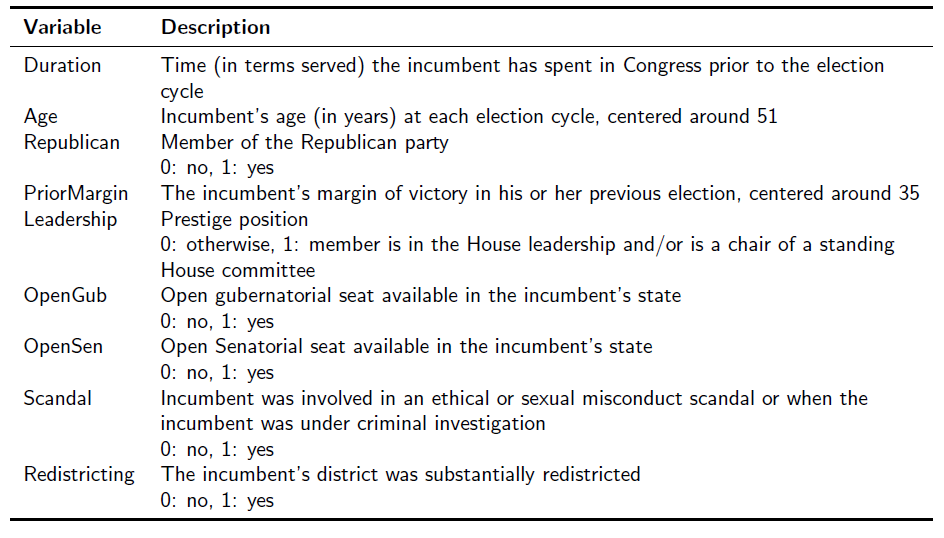
\includegraphics[width=\linewidth]{Table1.png}
        \end{table}
        \paragraph{}We fitted a penalized multinomial logit model with risks defined by cause 1 (General), 2(Primary), 3 (Retirement) and 4 (Ambition). The effect of covariates in the model $\lambda_r(t|\mathbf{x}) = \frac{ \exp{ ( \eta_{itr} ) } }{ 1+ \sum_{s=1}^{m} \exp{ (\eta_{its}) }  }$ is specified by the cause-specific linear predictors $\eta_{itr} = \beta_{0tr}+\mathbf{x}^\mathsf{T} \mathbf{\gamma_r}$All covariates described in Table \ref{Table1} are incorporated in the predictors. Moreover, we included all pairwise interactions with the exception of  Republican: Leadership, Leadership:Redistricting, Opengub:Scandal, Scandal:Redistricting because too few observations of the corresponding combinations are in the data. Such a high-dimensional interaction model cannot be properly handled by unpenalized ML estimation but stable estimation and efficient variable selection is obtained by using penalization. 
        \paragraph{} Since the adaptive version of the penalty yielded better cross-validation score, adaptive weights were used. Tuning parameters $\xi_1$ and $\xi_2$ were chosen on a $2$-dimensional grid by $5$-fold cross validation with the predictive deviance as loss criterion. The resulting tuning
        parameters were $\xi_1 = 6.0$ and $\xi_2 = 2.64$. For a fixed model, the corresponding cross validation score is shown in Figure \ref{Figure1}
        , where the vertical black dashed line marks the chosen tuning parameter.
        \begin{figure}[H]
            \centering
            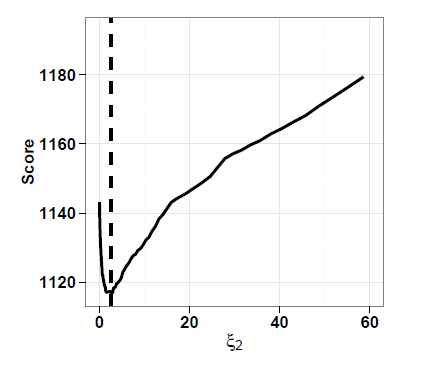
\includegraphics[scale=0.7]{./Figure1.png}
            \caption{Cross validation score subject to penalty parameter $\xi_2$ for $\xi_1 = 6.0$ for the Congressional career data}
            \label{Figure1}
        \end{figure}
        \paragraph{}Figure \ref{Figure2} shows the parameter estimates for the cause-specific time-varying baseline effects. The corresponding pointwise confidence intervals, marked by light-gray dashed lines, have been estimated by a nonparametric bootstrap method as proposed by Efron(1979) with 1000 bootstrap replications of the fitted model (i.e. fixed tuning parameters
        across bootstrap samples). It can be seen that cause-specific baseline effects are necessary because the shapes are quite different. 
        \begin{figure}[]
            \centering
            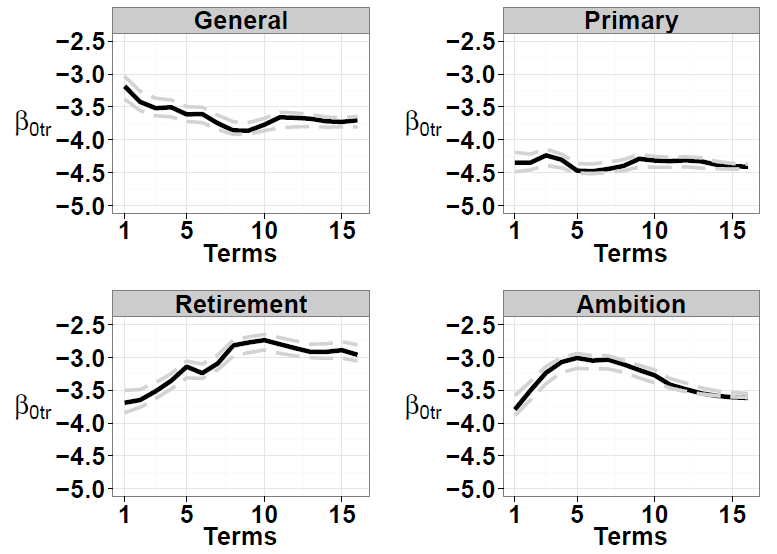
\includegraphics[scale=0.7]{./Figure2.png}
            \caption{Parameter estimates of the cause-specific time-varying baseline effects for the
                Congressional careers data. Dashed lines represent the $95\%$ pointwise bootstrap interval}
            \label{Figure2}
       \end{figure} 
       \paragraph{}Parameter estimates of the covariate effects are summarized in Table \ref{Figure2}. It shows the ordinary ML estimates and the estimates resulting from the penalized competing risk model with their corresponding standard errors. The computation of the standard errors is based on the empirical standard deviation of the respective coefficient across 1000 nonparametric bootstrap samples. It is immediately seen that the penalization removes a considerable number of effects, that is, only 68 out of 128 parameters remain in the model, leading to a strong reduction of the model complexity. 
       \begin{figure}
           \centering
           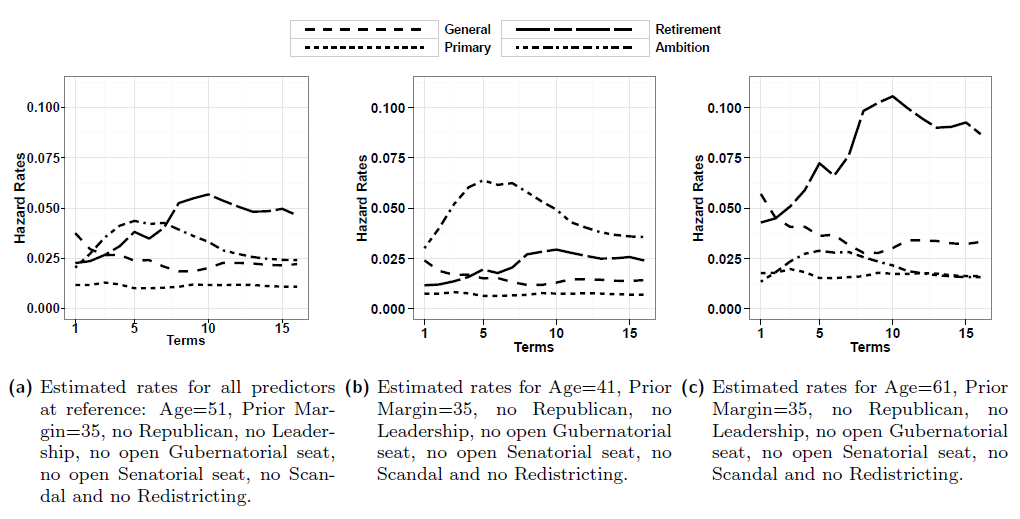
\includegraphics[width=\linewidth]{./Figure3.png}
           \caption{Estimated cause-specific hazard rates over time for the Congressional careers data}
            \label{Figure3}
       \end{figure} 
       \paragraph{}In Figure \ref{Figure3}a a selection of resulting hazard rates is depicted. It shows hazard functions for the following covariate characteristics: Age = 51, prior margin = 35, no Republican, no Leadership, no open Gubernatorial seat, no open Senatorial seat, no Scandal and no Redistricting for the transitions to General, Primary, Retirement and Ambition. It can be seen that the probability of retirement tends to increase over early terms and then remains rather stable.
       \paragraph{}The probability for seeking an alternative office as compared to reelection increases for early terms and then decreases. The hazard rates for losing either a primary or a general election are rather constant in the considered group. Figure \ref{Figure3}b and c show the hazard rates respectively for
       younger (Age = 41) and older (Age = 61) Congressmen compared to the reference group (Age = 51), while everything else remains unchanged. Younger Congressmen prefer to seek an alternative office and they do not intend to retire. For older Congressmen, the probability of retirement compared to reelection strongly increases. Moreover, the probability of losing either a primary or a general election is larger than in the reference group.
       \paragraph{}The selection effect is visualized by coefficient paths. In Figure \ref{Figure4} we show only the paths for the main effects. Each path indicates the penalized estimates subject to tuning parameter $\xi_2$, where the abscissa is transformed by $log(1+\xi_2)$). The paths illustrate how the estimates changes towards zero for increasing $\xi_2$. Hence, they show the effects of covariates on the terminating events when penalization is increased. The dashed black line indicates the value of  $\xi_2$ that was chosen via cross-validation.
       \begin{figure}
           \centering
           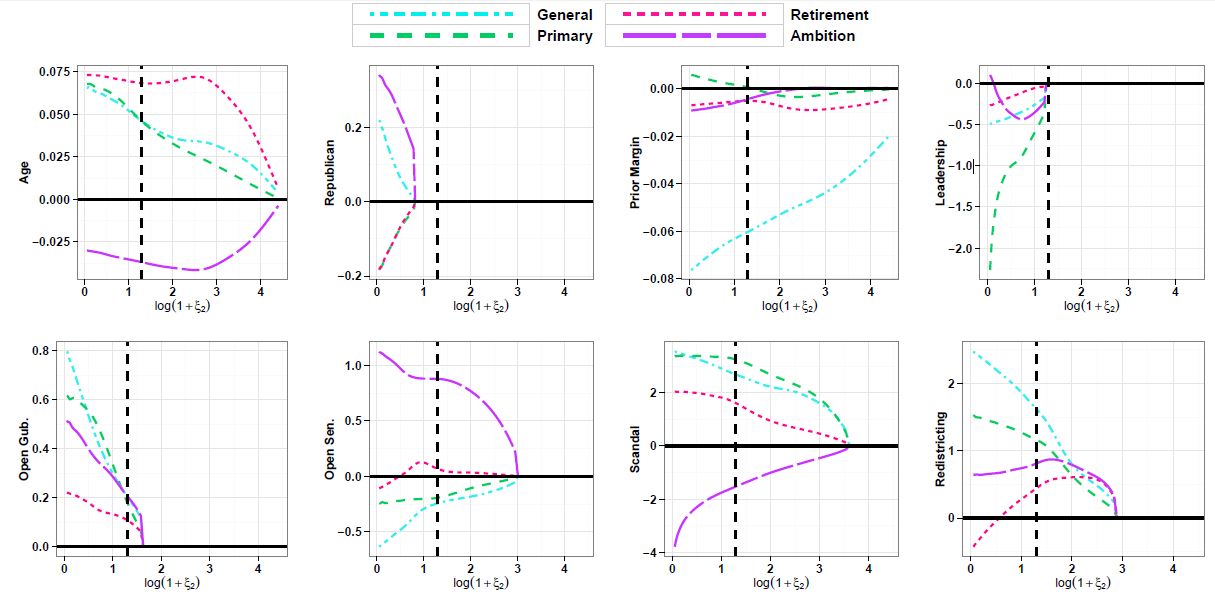
\includegraphics[width=\linewidth]{./Figure4.png}
           \caption{Coefficients paths of the main effects for the Congressional career data}
           \label{Figure4}
        \end{figure} 
       
        
    \section{Discussion}
        \paragraph{}In competing risk models for discrete duration time, one is interested in the the causespecific hazard rates. When modeling these cause-specific hazard rates, each explanatory
        variable is linked to a group of parameters. The proposed penalization method enforces the simultaneous shrinkage of parameters belonging to such a group. A parameter group even can be completely removed from the model yielding variable selection instead of parameter selection. Moreover, the proposed method allows that parameters representing the cause-specific baseline hazards vary over time. In order to avoid that adjacent parameters of the baseline effects have completely different values, an additional penalty term is incorporated that steers the smoothness of the baseline effects.
\end{document}